\documentclass[a4paper]{usiinfbachelorproject}

\captionsetup{labelfont={bf}}
%%%%%%%%%%%%%%%%%%%%%%%%%%%% PACKAGES %%%%%%%%%%%%%%%%%%%%%%%%%%%%%
\usepackage{float}
\usepackage{amsmath}

%%% Main Body %%%

\author{Costanza Rodriguez Gavazzi}

\title{\textbf{How do children search?}}
\subtitle{A tool to support researchers in understanding how children search for information online}
\versiondate{\today}

\begin{committee}

\advisor[Universit\`a della Svizzera Italiana, Switzerland]{ }{Monica }{Landoni }

\coadvisor[Universit\`a della Svizzera Italiana, Switzerland]{ }{Diletta Micol}{Tobia}

\end{committee}

\abstract { Abstract goes here ...

Things to write: Context, Problem, Limitations in SOA, Contribution and Findings
\vspace{0.5em}

\textbf{Keywords}:
% You may include up to six keywords or phrases. Keywords should be separated with semicolons. 

}

\begin{document}
\maketitle
\tableofcontents
%\listoffigures\newpage

\newpage
%%%%%%%%%%%%%%%%%%%%%%%%%%%% INTRODUCTION %%%%%%%%%%%%%%%%%%%%%%%%%%%%%
\section{\textbf{Introduction}}

Things to write in the introduction:
Acknowledge seminal work in the area (very similar tool or research).
In the last paragraph list all your contributions.
Add a subsection titled “Report structure” where you briefly discuss the content of each following section (e.g., In section 2, we review previous studies in the context of ….).

Context, Problem, Limitations in SOA, Contribution and Findings

\newpage

%%%%%%%%%%%%%%%%%%%% BACKGROUND AND RELATED WORK %%%%%%%%%%%%%%%%%%%%%
\section{\textbf{Background and Related Work}}

The study of how children search for information online is a growing area that connects education, information retrieval (IR), and human-computer interaction (HCI). The goal of this project was to develop a research tool that could collect rich interaction data from children using both traditional search engines and large language models (LLMs). Unlike other projects focused mainly on improving user experience or visual design, this project was designed as a flexible platform to support various research questions on children's search behaviors. At the same time, the tool had to be engaging and appropriate for younger users.

\subsection{Foundation}

The starting point for this project was the bachelor thesis by Savoia \cite{Savoia2025}. In her work, she proposed an interactive game designed to observe how children search for information. The interface was structured around a group of six islands, where each island represented a question framed with a specific emotional tone (positive, neutral, or negative). The children were allowed to choose how they wanted to answer the question, using a familiar web search interface (Google) or a chatbot-style LLM. Her work demonstrated that this narrative approach could encourage natural interactions and meaningful behavior from children.

Although her prototype successfully demonstrated the idea, it was not built with reuse or extensibility in mind but as a proof of concept. This project rebuilt the system from scratch to make it modular, maintainable, and suitable for future research experiments. Still, it kept the core idea of gameplay and the use of emotionally charged questions and flexibility in tool choice to support various search strategies.

\subsection{Motivation}

A review of the literature highlighted the need for a research tool tailored to children’s needs. Children are frequent users of search engines, especially in school settings, but often struggle to find relevant information efficiently \cite{Aliannejadi2021}. Most commercial tools like Google or Bing are designed for adults \cite{Aliannejadi2021, Landoni2021}, and there is no single search interface that fits all users, especially young people with different cognitive and emotional needs \cite{Landoni2021}.

In the IR research community, there is a clear call for child-friendly systems that are more suitable in educational contexts \cite{Landoni2020}. However, building such systems is challenging. Designing for children means taking into account their specific abilities: cognitive, technical, emotional and motor \cite{Chen2022}. In many cases, children say they want one thing, but their actual behavior shows something else. This is why relying only on interviews or post-task questionnaires can be misleading \cite{Aliannejadi2021}.

Unfortunately, children are often left out of mainstream IR research and there is a lack of reliable data on how they really use search tools \cite{Savoia2025}. Researchers have highlighted the need for dedicated datasets, experimental tools, and evaluation methods designed for children \cite{Landoni2021c}.

Observing how children search and interact with systems, we can gather important insights that help improve the design of future tools \cite{Savoia2025}. These insights can also guide the development of features that help children, for example, by offering visual cues to highlight relevance or reduce confusion \cite{Landoni2021}. Data from such tools can support many different research directions, including how emotions impact search performance, how children respond to positive or negative task framing, or how task complexity affects engagement \cite{Landoni2020, Landoni2021c}.

It is also interesting to consider how negative emotions are handled. Some research suggests that tracking negative user emotions could support better filtering, while others warn that hiding negative content might limit learning opportunities \cite{Landoni2020}.

A game-based tool, like the one built in this project, can collect structured data such as query logs, number of queries, time spent, and user clicks \cite{Aliannejadi2021}. It can also capture richer information about how children switch between tools or how many queries / prompts they need before answering. This kind of data would be difficult to gather with traditional observational methods or surveys.


\newpage

%%%%%%%%%%%%%%%%%%%%%%%%%%%% REQUIREMENTS %%%%%%%%%%%%%%%%%%%%%%%%%%%%%
\section{\textbf{Requirements}}

This project did not begin with a fixed specification. Instead, requirements emerged iteratively through exploration of the research domain, analysis of related literature, and discussions with the advisors. The system was designed to be general enough to support a wide variety of research questions in information retrieval (IR) and human-computer interaction (HCI), while also being engaging and usable for children.

The main objective was to implement a fully functional and reusable prototype capable of collecting detailed data on how children use traditional search engines and large language models (LLMs). The project builds on and extends Savoia's prototype \cite{Savoia2025}, which demonstrated the potential of a game-based framework to study children's search behavior but did not actually integrate the data collection aspect of it. \\
\linebreak
To structure the design, the following questions guided the requirements definition process:
\begin{itemize}
    \item What kind of data do researchers want to collect?
    \item Can a game-based interface be used to collect these data effectively?
    \item What kind of game design is both engaging and suitable for structured data collection?
    \item How can the tool remain usable and appealing to children?
    \item How can the system be modular, extensible, and maintainable for future research?
    \item How can it adapt to different experimental setups or research contexts?
\end{itemize}

These reflections acted as a guide to explore the literature, which then led to a concrete list of functional and non-functional requirements, discussed below.

\subsection{Data for Research Use}

Exploring the literature revealed that researchers need a wide range of data to understand children's search behaviors. This includes both quantitative metrics and qualitative observations. The following types of data were identified as relevant for this project:

\begin{itemize}
    \item \textbf{Query Logs:} Query text, number of queries, and tool usage data \cite{Aliannejadi2021, Savoia2025}.
    \item \textbf{Performance Indicators:} Session length, query term counts, click counts, and rank depth \cite{Landoni2021c}.
    \item \textbf{Task Outcome Data:} Final responses, with the idea that scoring based on teacher rubrics or predefined relevance criteria could be done later, when analyzing the gathered data \cite{Landoni2021c}.
    \item \textbf{Tool Preference:} Children’s selection patterns between search engine and LLM \cite{Savoia2025}.
    \item \textbf{Timing Data:} Time spent on each question, delays before interaction, etc. \cite{Savoia2025}.
\end{itemize}


\subsection{UI Insights from Literature}

Key research informed the requirements:

\begin{itemize}
    \item There is no one-size-fits-all SERP interface suitable for children \cite{Landoni2021}.
    \item Children prefer playful and engaging tools, and emotional design improves product recognition and user satisfaction \cite{Chen2022, Amin2022}.
    \item Humanized design elements such as avatars, animations, and storytelling are particularly effective for younger users \cite{Amin2022, Chen2022}.
    \item There is a need for tools that can capture structured data such as query logs, tool preferences, click behavior, on top of qualitative engagement metrics \cite{Savoia2025, Landoni2021c}.
    \item Participatory design methods show that children prefer familiar, usable UI elements but appreciate fun, cartoonish visuals \cite{Tapola2022, Landoni2021b}.
    \item Based on their age and cognitive abilities, children require different levels of scaffolding and support in search tasks \cite{Chen2022, Tapola2022, Amin2022}. In particular:

          \begin{itemize}

              \item \textbf{Ages 6 to 8:} Children in this group begin to mature and expand their vocabulary. Interfaces should use simple, familiar words, and reward systems are effective in maintaining engagement. Bright colors are still encouraged.

              \item \textbf{Ages 9 to 12:} These users value autonomy and prefer interfaces that offer control rather than instructions. Feedback should be informative rather than directive. Colors can be more subdued, such as green, gray, and navy tones. They are generally more skilled at navigating websites and handling smaller UI elements.
          \end{itemize}

\end{itemize}

\subsection{Functional Requirements}

\begin{itemize}
    \item \textbf{Language and Initialization}
          \begin{itemize}
              \item The language of the game must be modular and easily changeable.
              \item A landing page must appear before the game starts to allow teachers or researchers to explain the rules.
              \item The game must be reset when a new language is selected.
          \end{itemize}

    \item \textbf{Session Management}
          \begin{itemize}
              \item Each session must be identified by a unique user code provided by the teacher.
              \item The game must start only after the user inputs a valid code.
              \item The game must persist its state on page refresh using local storage.
              \item Researchers must be able to download session data at any time, even if the game is incomplete.
              \item When downloading data, the system must request a password to protect the export.
          \end{itemize}

    \item \textbf{Gameplay Logic}
          \begin{itemize}
              \item The game must include six clickable islands, presented in a randomized order per session.
              \item Islands can be clicked in any order.
              \item Each island represents a question with a specific emotional framing: positive, neutral, or negative.
              \item Once answered, an island becomes inactive and cannot be clicked again.
              \item Inactive islands must show a different cursor, remove hover effects, and a message should appear when trying to click on them.
              \item Each completed island increases the score by 10 points (maximum 60).
              \item The current score must be shown at the top right of the screen.
          \end{itemize}

    \item \textbf{Search Tool Interfaces}
          \begin{itemize}
              \item Clicking on an island must open a question page where the user chooses between Google or Gemini (LLM).
              \item Users must be allowed to switch between the two tools freely before submitting an answer.
              \item The Google interface must visually mimic a real search engine and display the top 10 results.
              \item The Gemini interface must mimic a realistic chat interface.
              \item Clicking on a Google result must open the link in a new browser tab.
          \end{itemize}

    \item \textbf{User Interaction Tracking}
          \begin{itemize}
              \item The system must record per-island data:
                    \begin{itemize}
                        \item \texttt{question}, \texttt{sentiment}, \texttt{openTime}, \texttt{submitTime}
                        \item \texttt{choiceForAnswer}: sequence of tool switches
                        \item \texttt{Queries}: a list of objects containing information about each query or prompt performed by the user
                        \item \texttt{userAnswer}: the final answer
                    \end{itemize}
              \item The system must record per-session data:
                    \begin{itemize}
                        \item \texttt{gameLanguage}, \texttt{userCode}, \texttt{startTime}, \texttt{finishTime}, \texttt{sessionLength}
                        \item \texttt{islandCompletionOrder}, \texttt{islandClickOrder}
                        \item \texttt{totalClicksInSession}, \texttt{timeBeforeFirstClick}, \texttt{score}
                    \end{itemize}
          \end{itemize}

    \item \textbf{User Experience and Engagement}
          \begin{itemize}
              \item The game must allow revisiting of islands prior to submission.
              \item The emotional tone must be visually represented with colors or icons.
              \item The UI must balance playful and realistic design to reflect real-world behavior.
              \item Upon completion, a thank you page must show the user's final score.
              \item The background must include animations to enhance engagement.
          \end{itemize}
\end{itemize}


\newpage

%%%%%%%%%%%%%%%%%%%%%%%%%%%% SYSTEM DESIGN %%%%%%%%%%%%%%%%%%%%%%%%%%%%%
\section{\textbf{System Design}}


\newpage

%%%%%%%%%%%%%%%%%%%%%%%%%%%% CONCLUSIONS %%%%%%%%%%%%%%%%%%%%%%%%%%%%%

\section{\textbf{Conclusions}}

\subsection{\textbf{Usage Scenarios}}

This section illustrates how reaserchers or teachers can set up the game and dowload the data, and how a child interacts with it during a typical session.

\subsubsection*{\textbf{Step 1: Language Selection}}

The game begins with the language choice screen (Fig.~\ref{fig:language-choice}). The researcher or teacher selects their preferred language before continuing, setting up the game for the child. A hover effect provides visual feedback (Fig.~\ref{fig:language-hover}).

\begin{figure}[H]
    \begin{minipage}[b]{0.5\textwidth}
        \centering
        \includegraphics[width=0.9\textwidth]{figures/language-choice.png}
        \caption{Language choice screen.}
        \label{fig:language-choice}
    \end{minipage}%
    \hfill
    \begin{minipage}[b]{0.5\textwidth}
        \centering
        \includegraphics[width=0.9\textwidth]{figures/language-hover.png}
        \caption{Hover effect on language choice.}
        \label{fig:language-hover}
    \end{minipage}
\end{figure}

\subsubsection*{\textbf{Step 2: Session Start}}

The child sees the game start screen (Fig.~\ref{fig:start-page}), with a hover animation guiding them to begin (Fig.~\ref{fig:start-hover}).

\begin{figure}[H]
    \begin{minipage}[b]{0.5\textwidth}
        \centering
        \includegraphics[width=0.9\textwidth]{figures/start-page.png}
        \caption{Game start screen.}
        \label{fig:start-page}
    \end{minipage}%
    \hfill
    \begin{minipage}[b]{0.5\textwidth}
        \centering
        \includegraphics[width=0.9\textwidth]{figures/start-hover.png}
        \caption{Hover effect on start button.}
        \label{fig:start-hover}
    \end{minipage}
\end{figure}

\subsubsection*{\textbf{Step 3: Entering a Code}}

The system requires the child to enter the session code they received prior to the start of the session (Fig.~\ref{fig:code-check}), which is validated (Fig.~\ref{fig:code-ok}). This ensures all data is associated with a specific session.

\begin{figure}[H]
    \begin{minipage}[b]{0.5\textwidth}
        \centering
        \includegraphics[width=0.9\textwidth]{figures/code-check.png}
        \caption{Session code entry screen.}
        \label{fig:code-check}
    \end{minipage}%
    \hfill
    \begin{minipage}[b]{0.5\textwidth}
        \centering
        \includegraphics[width=0.9\textwidth]{figures/code-ok.png}
        \caption{Successful code validation.}
        \label{fig:code-ok}
    \end{minipage}
\end{figure}

\subsubsection*{\textbf{Step 4: The Island Map}}

The core game component corresponds to the map page (Fig.~\ref{fig:map}). Each of the six clickable islands represents a unique search task. Hover feedback (Fig.~\ref{fig:map-hover}) helps guide children’s attention.


\begin{figure}[H]
    \begin{minipage}[b]{0.5\textwidth}
        \centering
        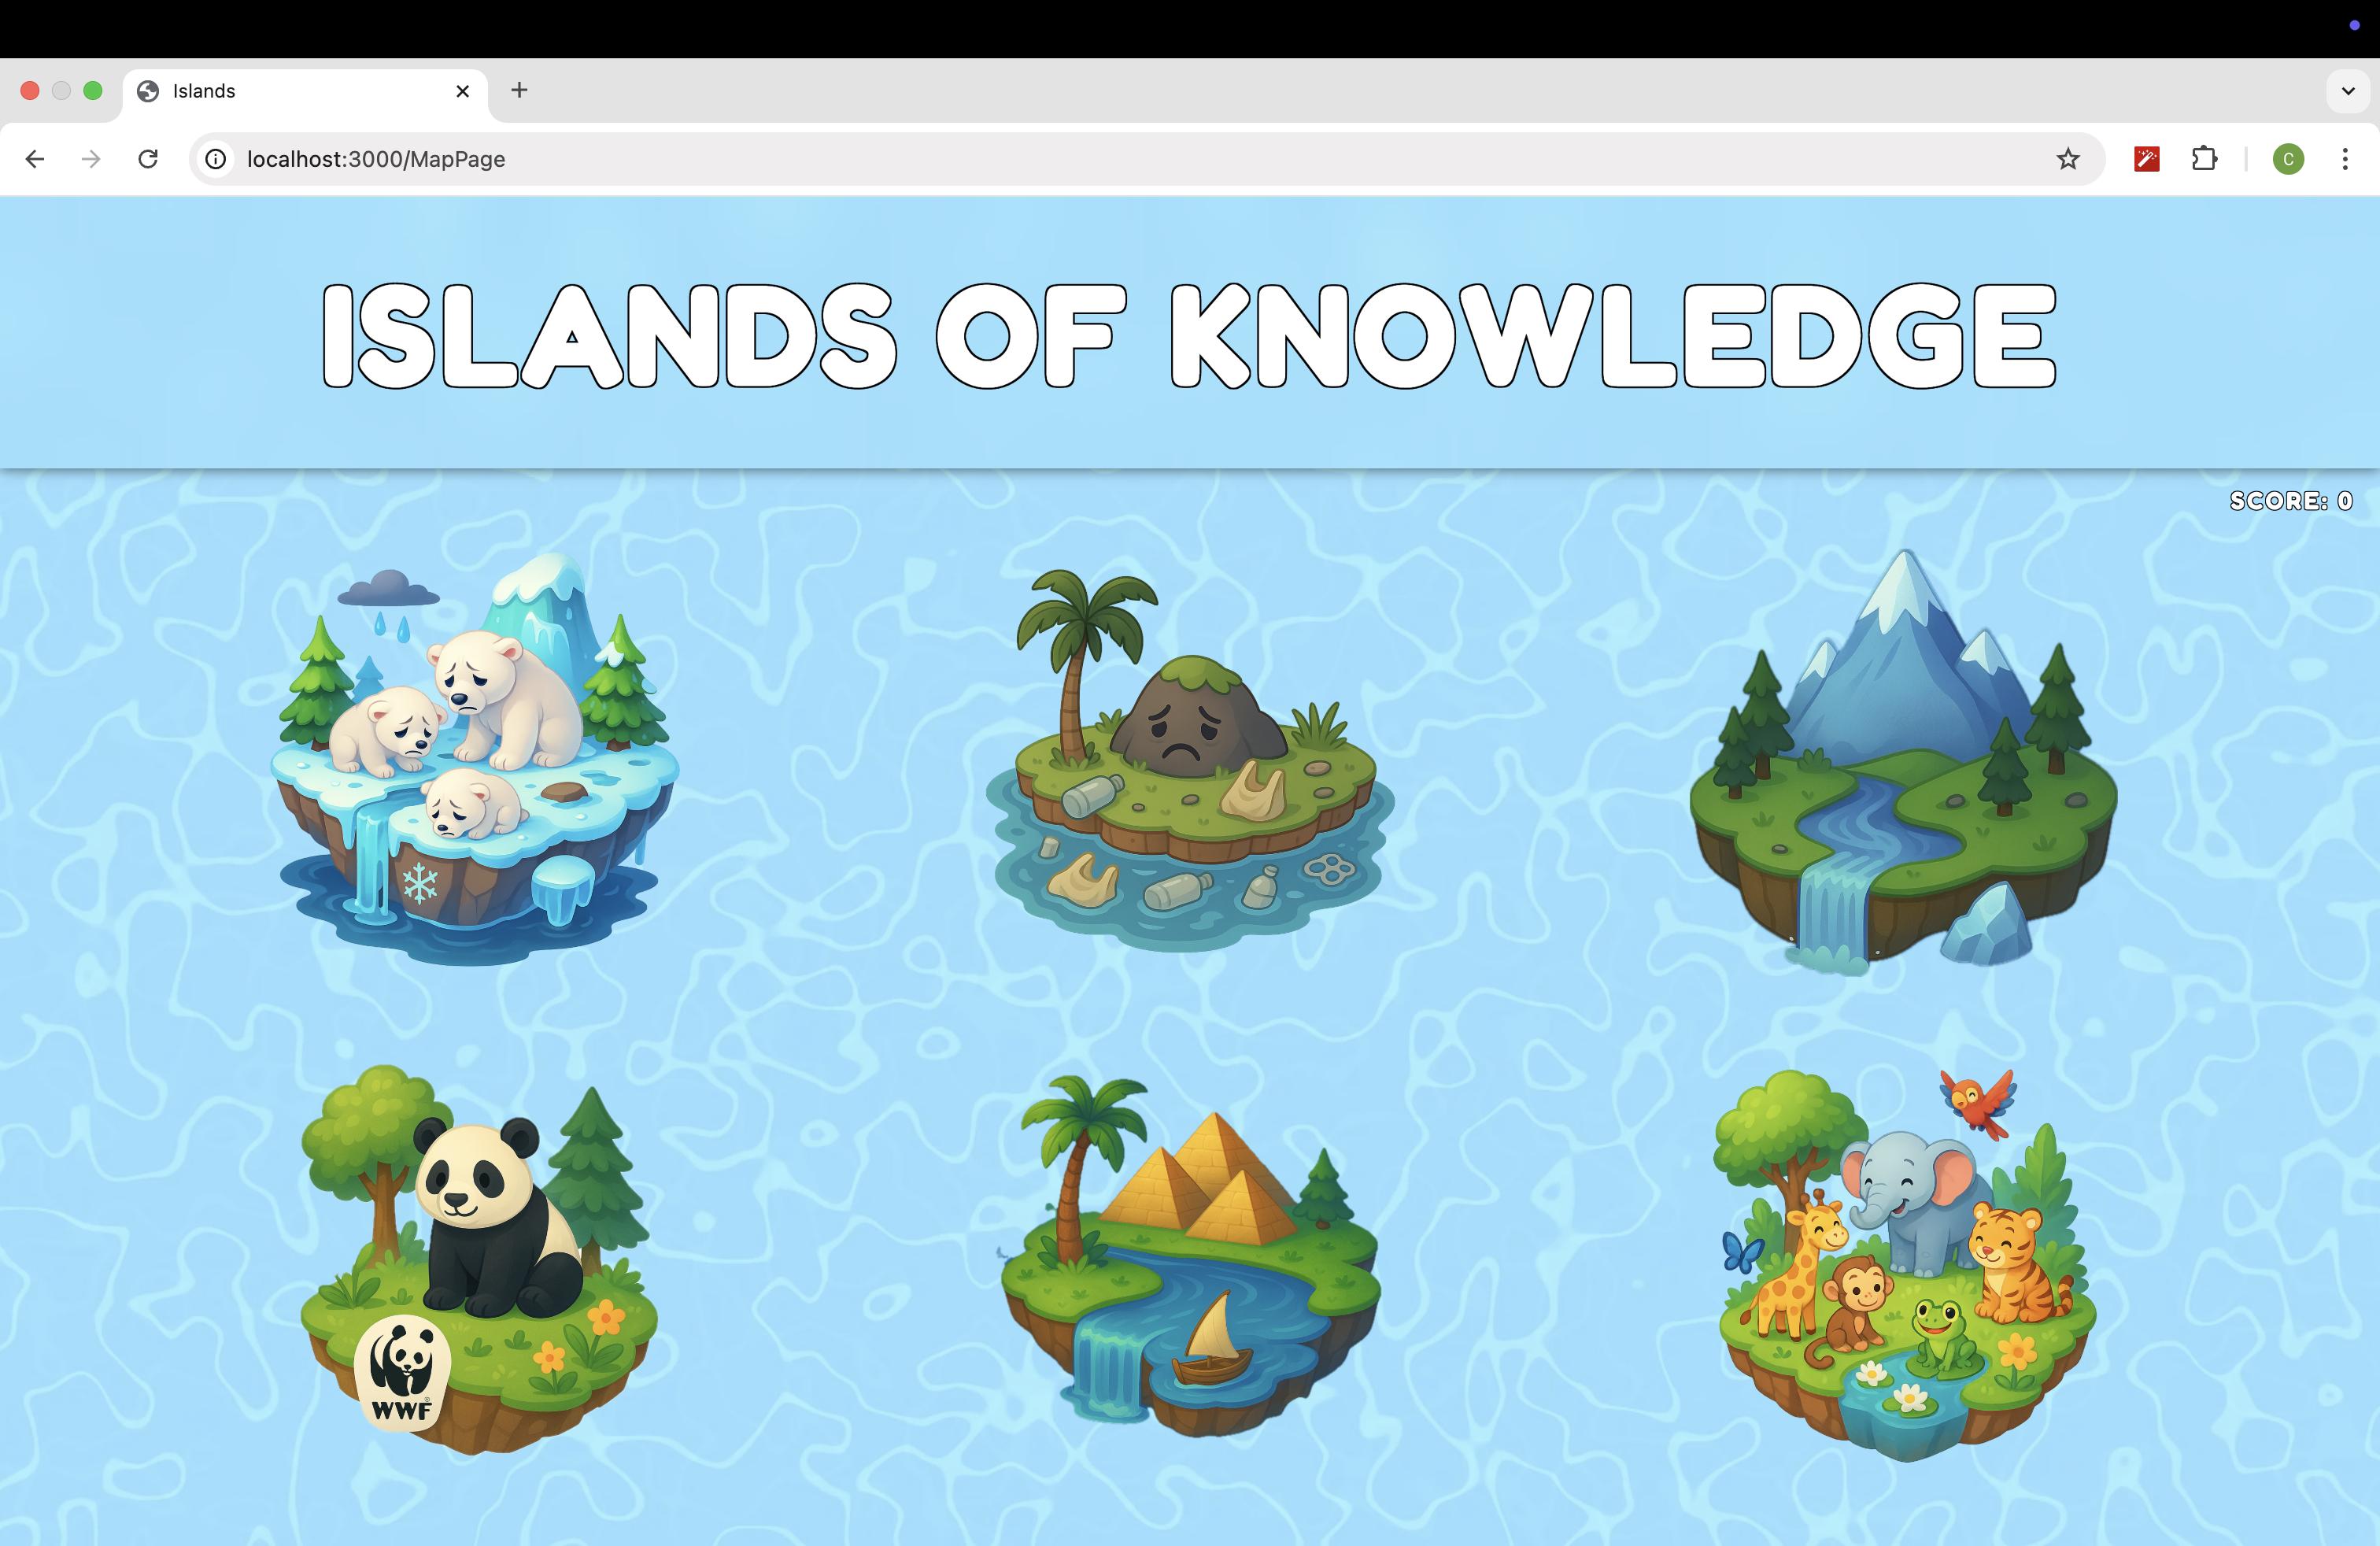
\includegraphics[width=0.9\textwidth]{figures/map.png}
        \caption{Island map with clickable islands.}
        \label{fig:map}
    \end{minipage}%
    \hfill
    \begin{minipage}[b]{0.5\textwidth}
        \centering
        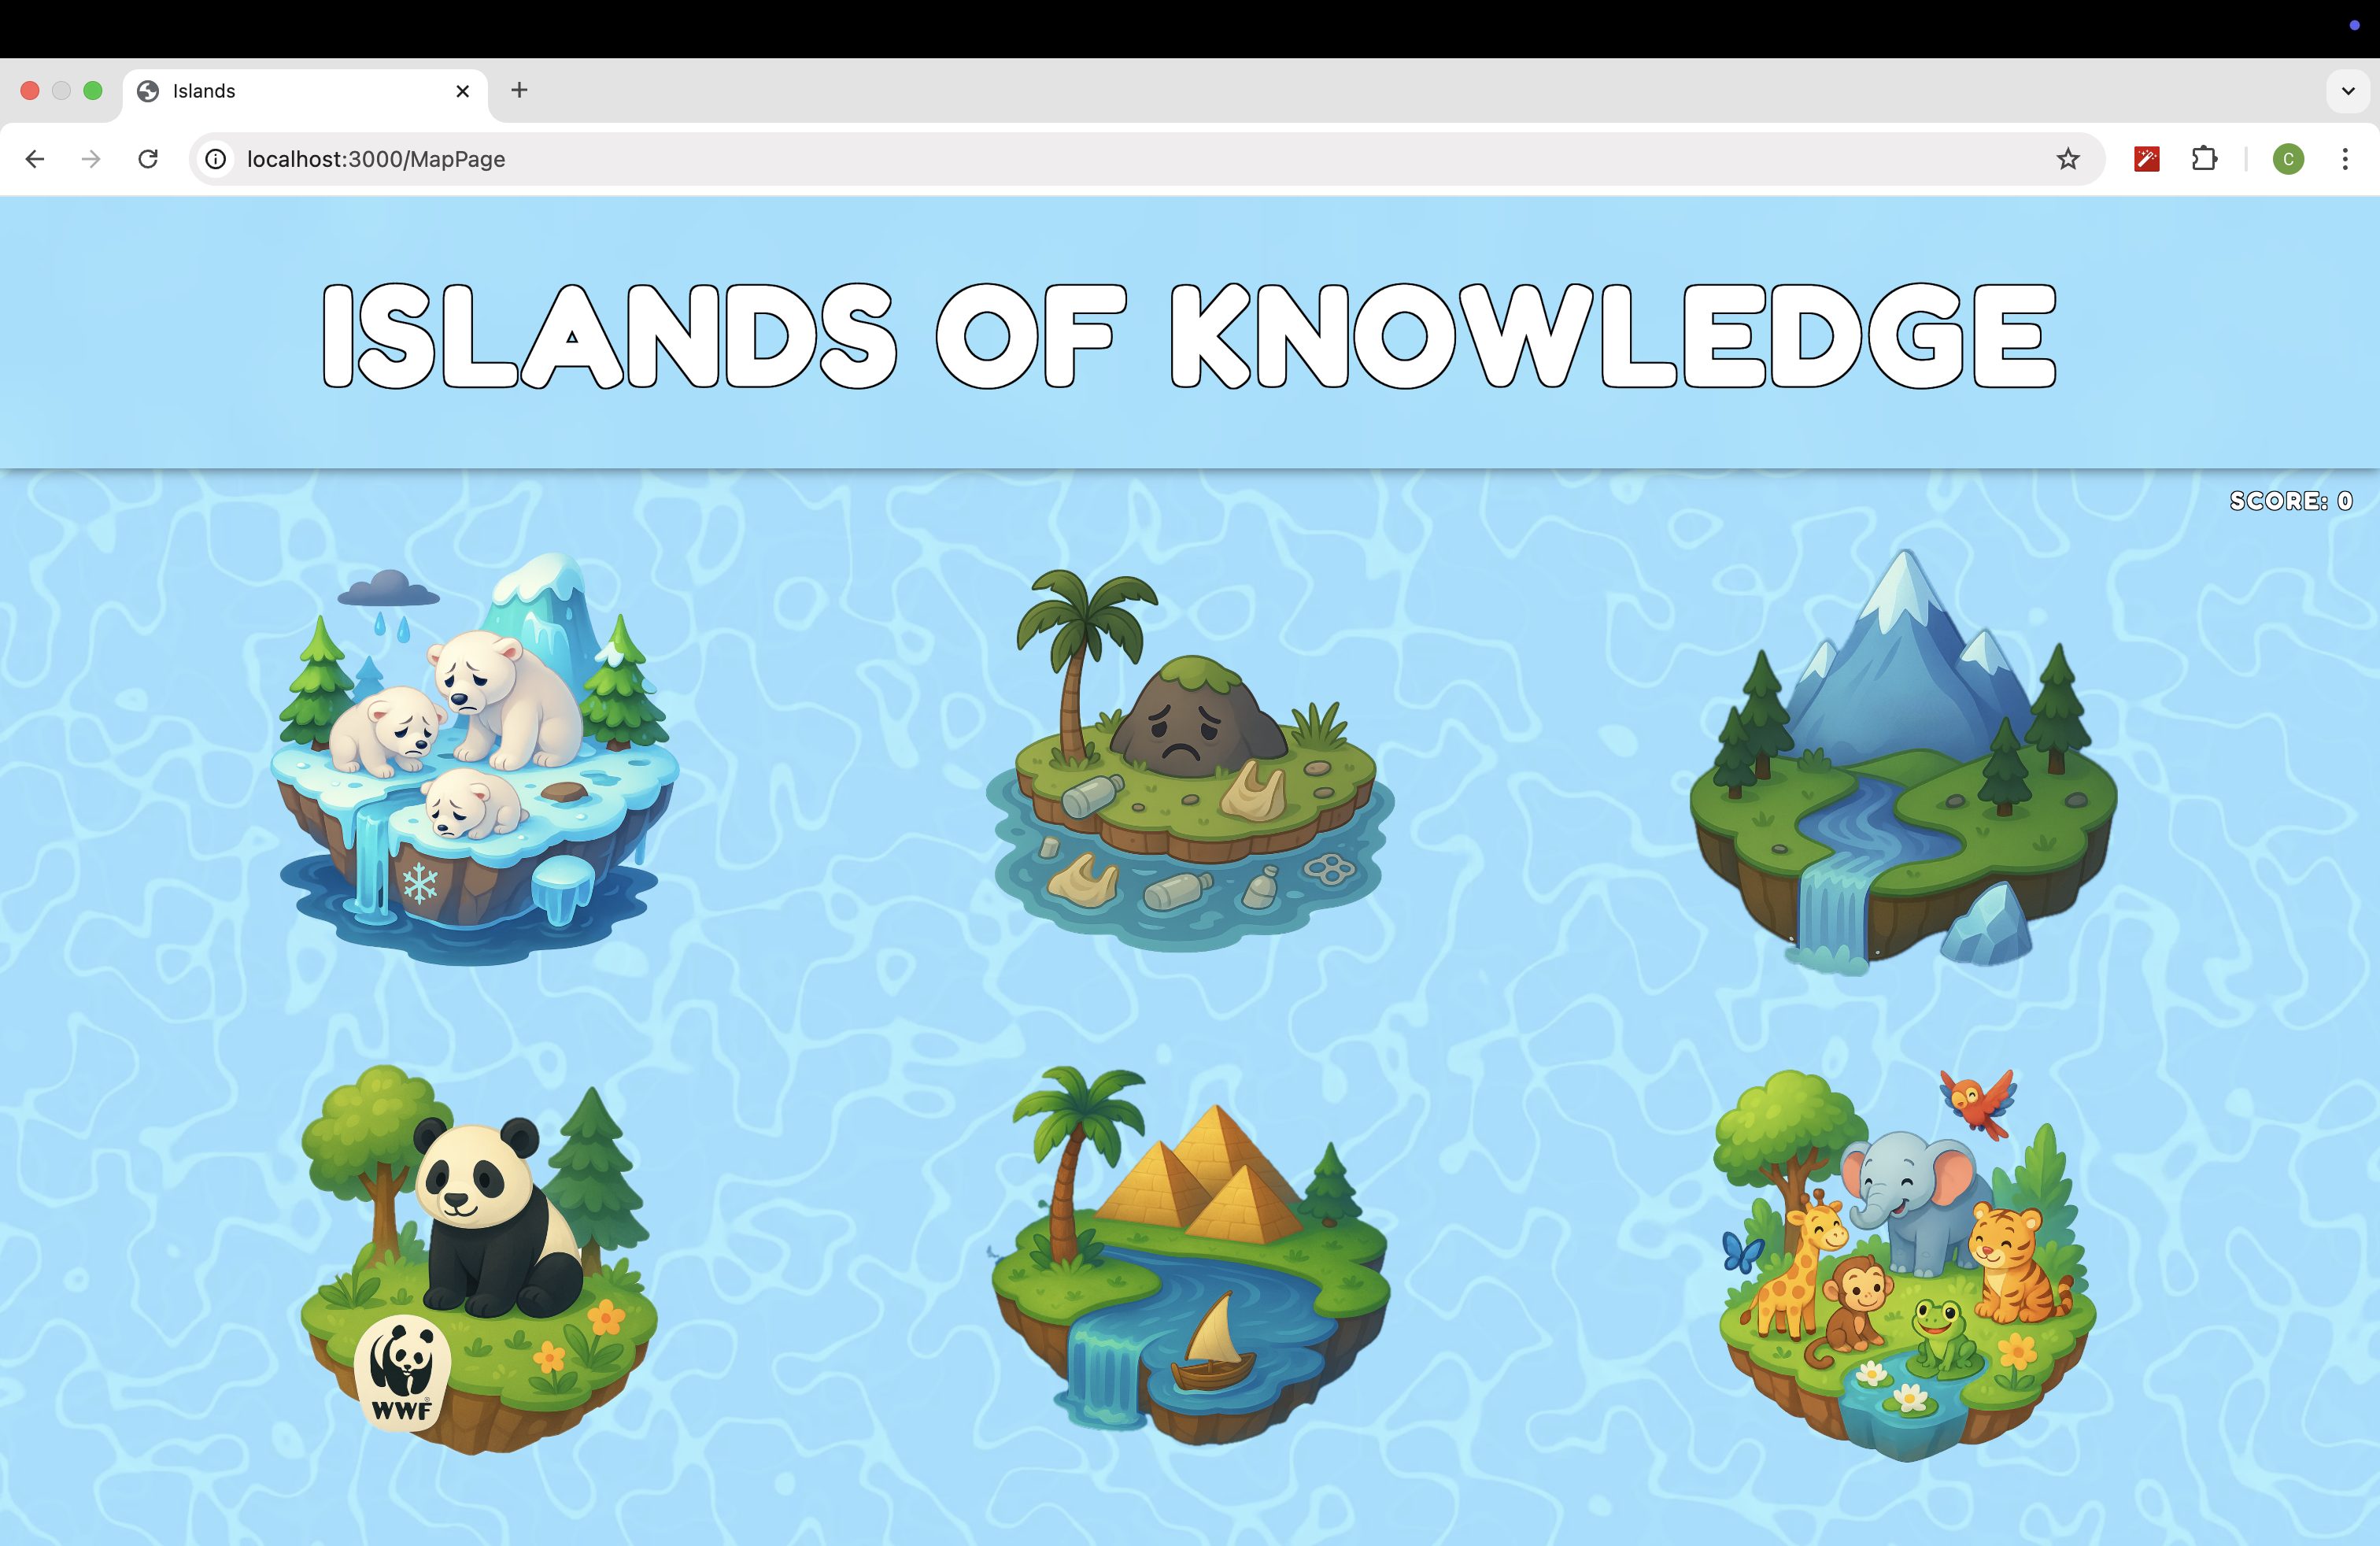
\includegraphics[width=0.9\textwidth]{figures/map-hover.png}
        \caption{Hover effect on islands.}
        \label{fig:map-hover}
    \end{minipage}
\end{figure}

\subsubsection*{\textbf{Step 5: Tool Choice}}

After selecting an island, the child reaches a tool selection page (Fig.~\ref{fig:choice-page}) where they choose between a traditional search engine (Google) and a large language model (Gemini).

\begin{figure}[H]
    \centering
    \includegraphics[width=0.5\textwidth]{figures/choice-page.png}
    \caption{Tool choice screen.}
    \label{fig:choice-page}
\end{figure}

\subsubsection*{\textbf{Step 6: Using Google}}

If the child selects Google, they are presented with a simulated SERP (Fig.~\ref{fig:google}). Clicking on links (which open in a new tab) mimics realistic search behavior (Fig.~\ref{fig:serp}). Links are opened in a new tab.

\begin{figure}[H]
    \begin{minipage}[b]{0.5\textwidth}
        \centering
        \includegraphics[width=0.9\textwidth]{figures/serp.png}
        \caption{Google search results with clickable links.}
        \label{fig:serp}
    \end{minipage}%
    \hfill
    \begin{minipage}[b]{0.5\textwidth}
        \centering
        \includegraphics[width=0.9\textwidth]{figures/google.png}
        \caption{Simulated Google SERP.}
        \label{fig:google}
    \end{minipage}
\end{figure}

\subsubsection*{\textbf{Step 7: Using Gemini}}

Alternatively, children can choose Gemini, where a chat-like interface appears (Fig.~\ref{fig:gemini}). A waiting screen mimics LLM response delay after they submit a prompt (Fig.~\ref{fig:gemini-waiting}), followed by result output (Fig.~\ref{fig:gemini-results}).

\begin{figure}[H]
    \begin{minipage}[b]{0.5\textwidth}
        \centering
        \includegraphics[width=0.9\textwidth]{figures/gemini.png}
        \caption{Gemini chat interface.}
        \label{fig:gemini}
    \end{minipage}%
    \hfill
    \begin{minipage}[b]{0.5\textwidth}
        \centering
        \includegraphics[width=0.9\textwidth]{figures/gemini-waiting.png}
        \caption{Waiting screen for Gemini response.}
        \label{fig:gemini-waiting}
    \end{minipage}
    \begin{minipage}[b]{0.5\textwidth}
        \centering
        \includegraphics[width=0.9\textwidth]{figures/gemini-results.png}
        \caption{Gemini response output.}
        \label{fig:gemini-results}
    \end{minipage}
\end{figure}

\subsubsection*{\textbf{Step 8: Submitting an Answer}}

After exploring results, the child can type a final answer (Fig.~\ref{fig:answer}). Once submitted, the island becomes inactive. If the child attempts to revisit a completed island, a warning is shown (Fig.~\ref{fig:warning}).

\begin{figure}[H]
    \begin{minipage}[b]{0.5\textwidth}
        \centering
        \includegraphics[width=0.9\textwidth]{figures/answer.png}
        \caption{Final answer submission screen.}
        \label{fig:answer}
    \end{minipage}%
    \hfill
    \begin{minipage}[b]{0.5\textwidth}
        \centering
        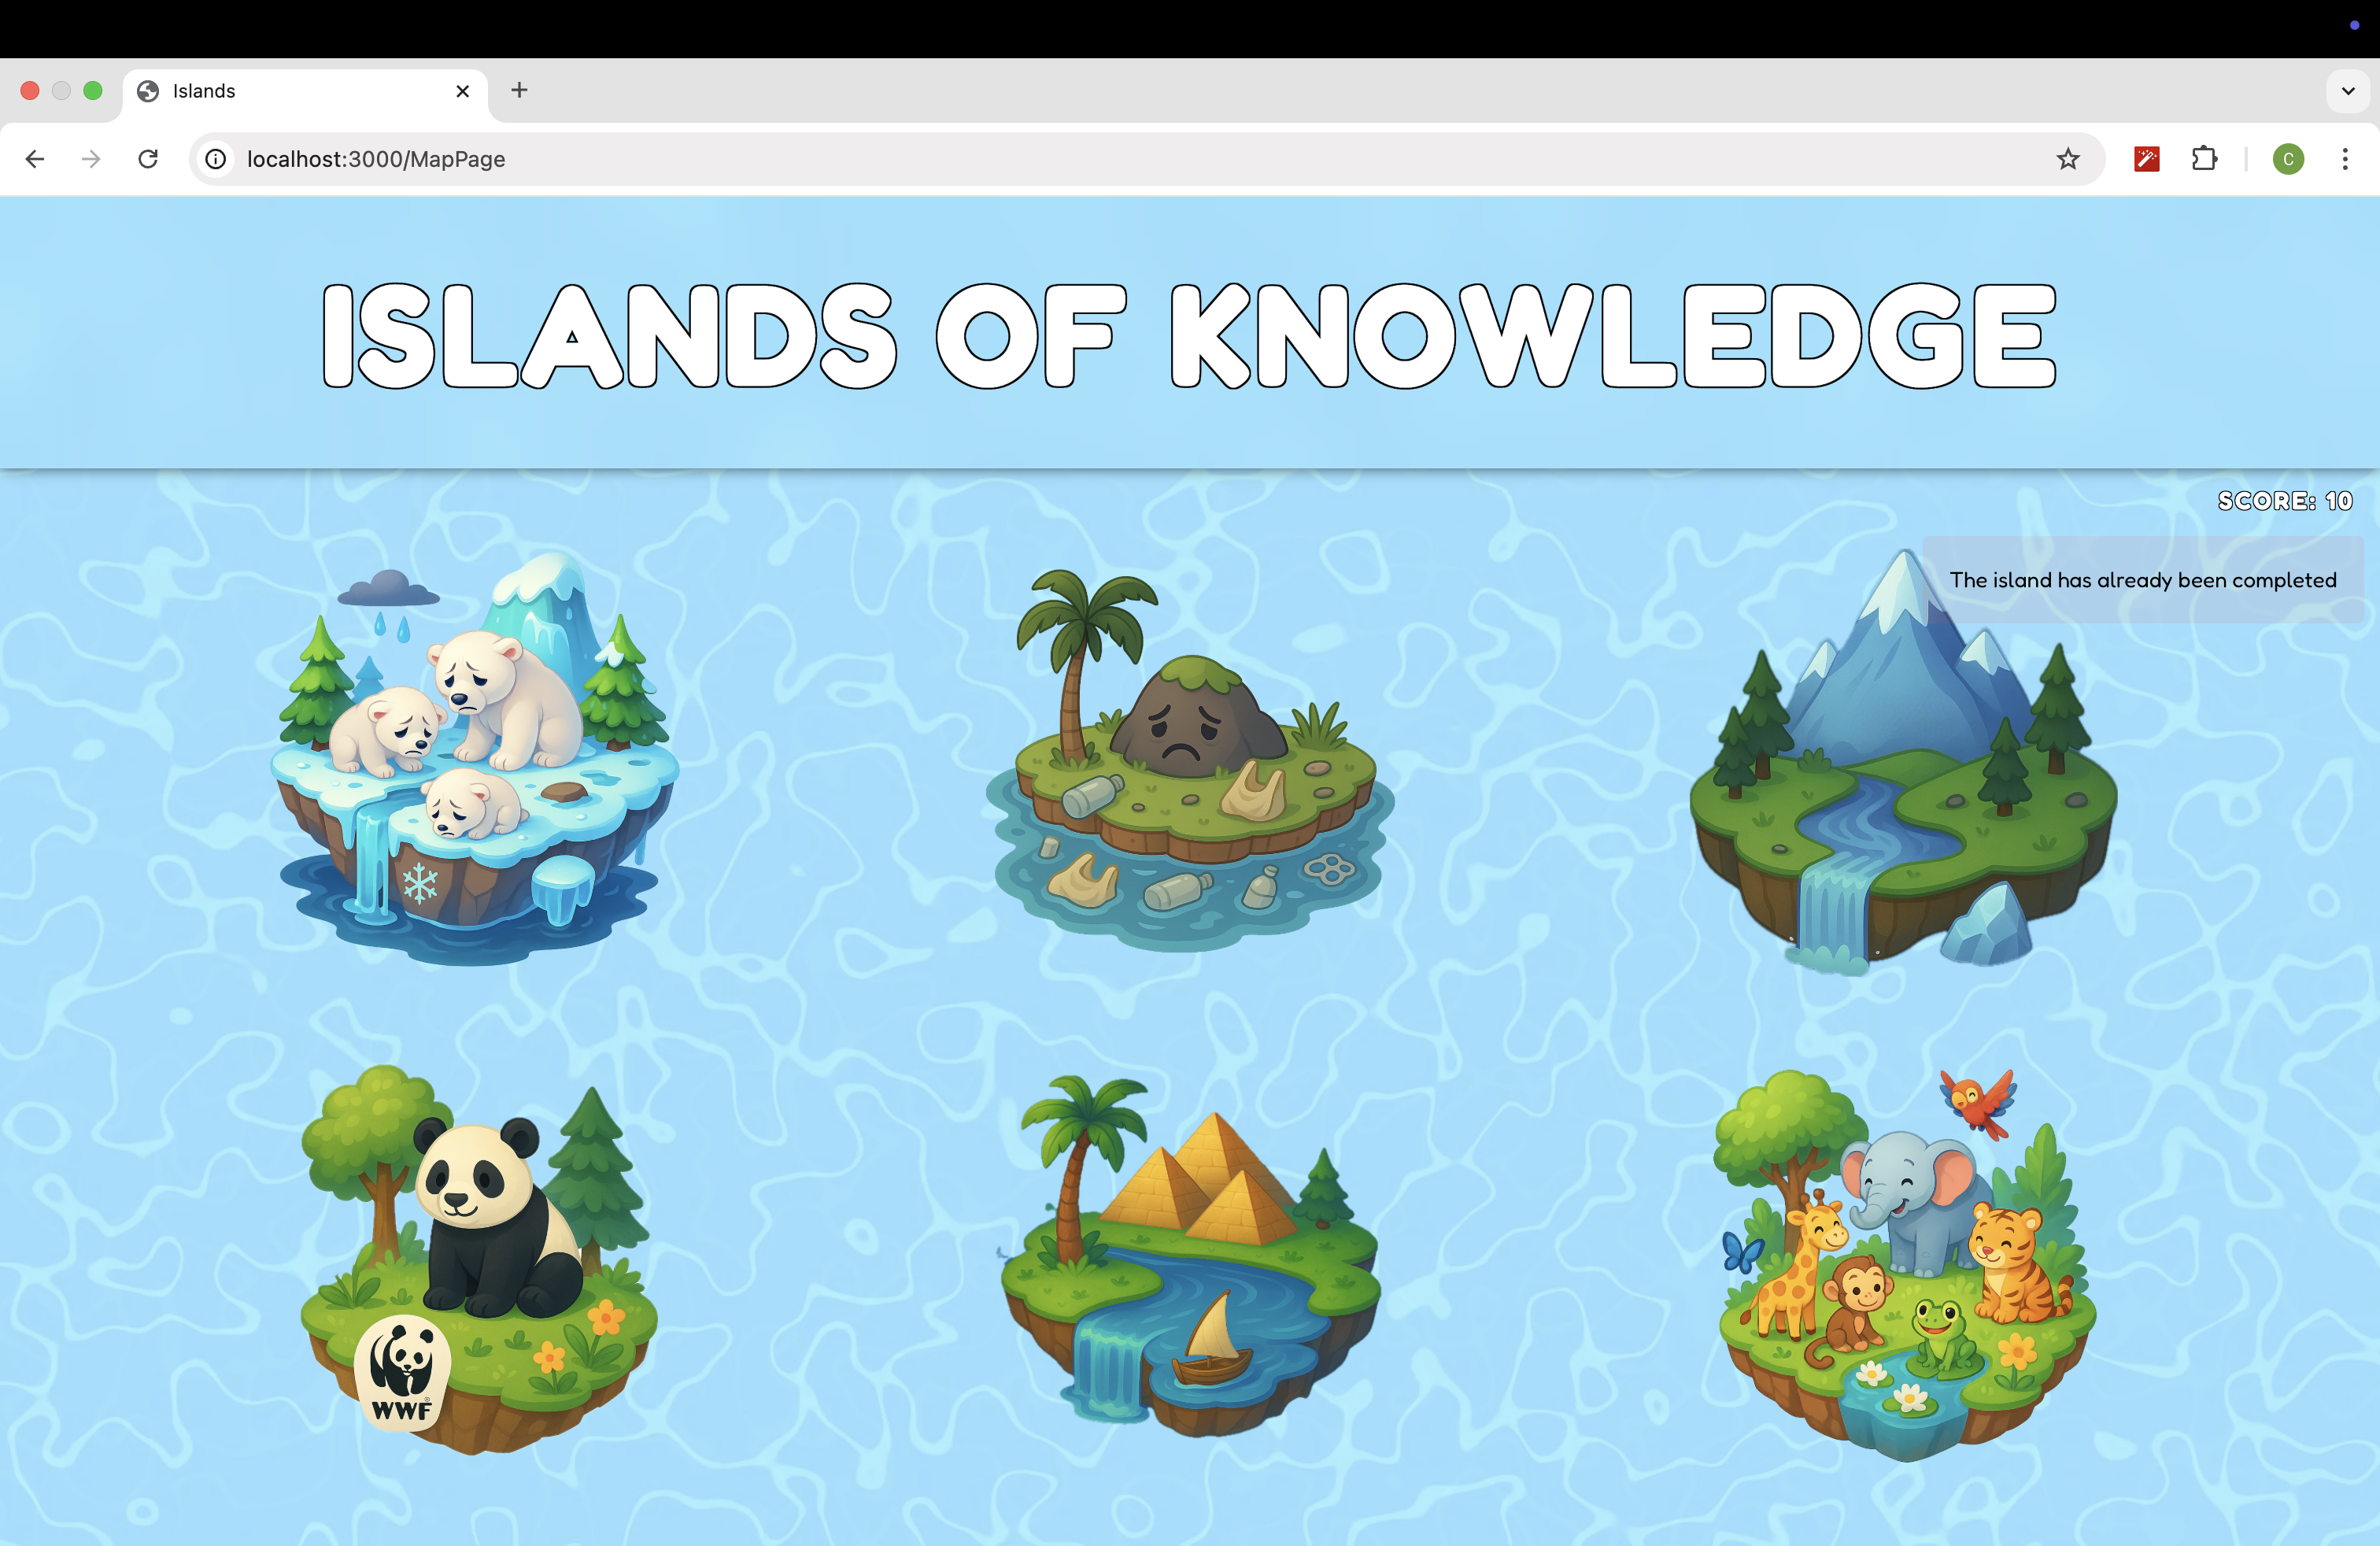
\includegraphics[width=0.9\textwidth]{figures/warning.png}
        \caption{Can't click on a completed island.}
        \label{fig:warning}
    \end{minipage}
\end{figure}

\subsubsection*{\textbf{Step 9: Final Page and Data Export}}

After completing all six islands, the child sees their final score (Fig.~\ref{fig:final-score}). Each island completed contributes 10 points, with a maximum of 60.

To end the session, a password-protected download prompt is shown (Fig.~\ref{fig:download}), allowing the teacher or researcher to save all session data locally. It was a design choice to use the brower's prompt functionality instead of a custom modal, to discourage children from trying to tamper with the data export.

\begin{figure}[H]
    \begin{minipage}[b]{0.5\textwidth}
        \centering
        \includegraphics[width=0.9\textwidth]{figures/final-score.png}
        \caption{Final score screen after completing all islands.}
        \label{fig:final-score}
    \end{minipage}%
    \hfill
    \begin{minipage}[b]{0.5\textwidth}
        \centering
        \includegraphics[width=0.9\textwidth]{figures/download.png}
        \caption{Password-protected data download prompt.}
        \label{fig:download}
    \end{minipage}
\end{figure}



\subsection{\textbf{Experts' Feedback}}

\subsection{\textbf{Future Work}}


\newpage

%%%%% BIBLIOGRAPHY %%%%%
\bibliographystyle{abbrv}
\bibliography{references}

\end{document}
